% Chapter 1

\chapter{Introducción general} % Main chapter title

\label{Chapter1} % For referencing the chapter elsewhere, use \ref{Chapter1} 
\label{IntroGeneral}

%----------------------------------------------------------------------------------------

% Define some commands to keep the formatting separated from the content 
\newcommand{\keyword}[1]{\textbf{#1}}
\newcommand{\tabhead}[1]{\textbf{#1}}
\newcommand{\code}[1]{\texttt{#1}}
\newcommand{\file}[1]{\texttt{\bfseries#1}}
\newcommand{\option}[1]{\texttt{\itshape#1}}
\newcommand{\grados}{$^{\circ}$}

%----------------------------------------------------------------------------------------

%\section{Introducción}

%----------------------------------------------------------------------------------------
En este capítulo se realiza una introducción a la realidad aumentada y los sistemas de control distribuidos. Hacia el final, se explica la motivación, alcance y objetivos del presente trabajo.

\section{Realidad Aumentada}
\subsection{Tecnología}

La digitalización del mundo real tiene distintos niveles. Podemos clasificarla en realidad virtual, realidad aumentada y realidad mixta, como puede verse en la figura \ref{fig:realidades}:

\begin{figure}[htpb]
	\centering
	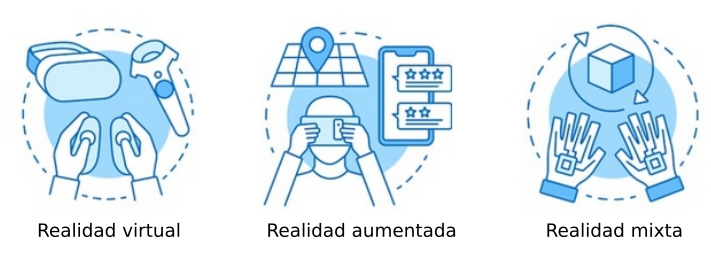
\includegraphics[width=\textwidth]{./Figures/realidades.png}
	\caption{Clasificación de tecnologías\protect\footnotemark.}
	\label{fig:realidades}
\end{figure}

\footnotetext{Imagen tomada de \url{https://scand.com/company/blog/augmented-mixed-and-virtual-reality-for-business/}}

La realidad virtual, consiste en un ambiente completamente digital. Se buscan aislar los sentidos del usuario del mundo real. De esta manera el usuario queda inmerso en otra realidad con la cual puede interactuar. Los dispositivos que permiten esta interacción son los cascos de realidad virtual y sus \textit{joysticks}.

La realidad aumentada es una tecnología que permite conectar los dos mundos, el mundo físico y el mundo digital. Esto se logra superponiendo imágenes sobre la percepción que tenemos del mundo real, mediante el uso de hologramas o incluso con teléfonos celulares. Donde al activar la cámara, nos muestra en la pantalla no solo el ambiente en el que estamos, sino que vemos proyectada información adicional. Ejemplos de esta tecnología, son los populares filtros de Instagram o el juego PokemonGo.

Por ultimo, la realidad mixta. Esta tecnología es una mejora de la realidad aumentada. Los elementos no solo son adicionados sobre la percepción visual, sino que interactúan ademas con el espacio físico. Por ejemplo, si tuviéramos una pelota en una aplicación de realidad mixta, la misma podría rodar cuesta abajo de una escalera.


\subsection{Procedimientos \textit{batch}}

Una operación \textit{batch} o por lotes es aquella en la cual las condiciones de operación cambian con el tiempo. Por lo general, se siguen una serie de pasos, el producto se transfiere a la siguiente fase de la operación, y el proceso comienza de nuevo. En la figura \ref{fig:tanks} podemos ver que en un proceso por lotes, solo cuando llegamos a t=4, obtenemos el producto final deseado:\\

\begin{figure}[htpb]
	\centering
	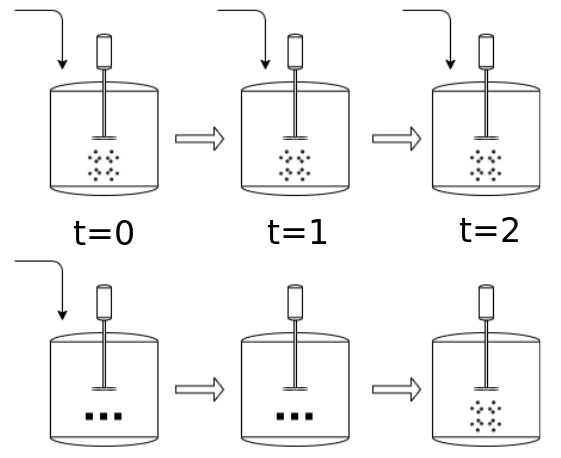
\includegraphics[scale=.45]{./Figures/tanks.png}
	\caption{proceso continuo (superior) vs. proceso por lotes (inferior)\protect\footnotemark.}
	\label{fig:tanks}
\end{figure}

Los procedimientos operativos para los procesos por lotes son generalmente más complicados y difíciles de escribir que para las instalaciones de estado estacionario porque el tiempo es un factor. Además, muchas instalaciones están diseñadas para fabricar varios productos a partir de los mismos equipamientos en diferentes momentos. Por lo tanto, se necesitan dos o más procedimientos para los mismos equipos de la planta, creando la posibilidad de confusiones y malentendidos.\\

Algunas operaciones por lotes implican el uso de hojas de cálculo. Por ejemplo, un operador puede agregar una bolsa de químicos a un reactor y luego agregar un segundo químico. La razón del segundo al primero debe ser exacta. El operador pesará la primera bolsa, calculará el peso del segundo químico necesario y procederá a pesar ese químico. Se necesita entonces una hoja de cálculo para determinar los requisitos para el peso del segundo producto.

\subsection{Sistemas de control distribuidos}

Los sistema de control distribuidos, también conocidos por sus siglas en ingles DCS. Son sistemas compuestos por sensores, controladores y computadoras que se distribuyen por toda la planta. Cada uno de estos elementos tiene un propósito único, como la adquisición de datos, el control de procesos, el almacenamiento de datos o la visualización gráfica. Estos elementos individuales se comunican con una sistema centralizado a través de la red de área local de la planta, denominada red de control. A continuación se muestra en la figura \ref{fig:800xA}, la arquitectura de red del sistema DCS de ABB, usado en este trabajo:

\begin{figure}[htpb]
	\centering
	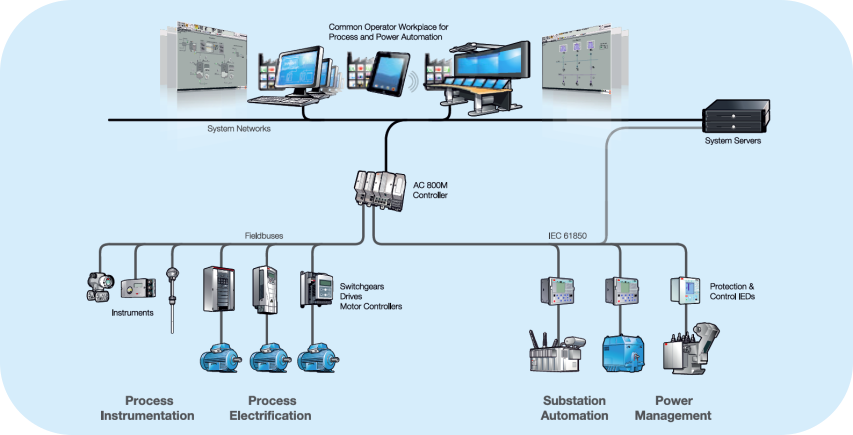
\includegraphics[width=\textwidth]{./Figures/800xA.png}
	\caption{Sistema de control distribuido 800xA\protect\footnotemark.}
	\label{fig:800xA}
\end{figure}

\footnotetext{Imagen tomada de \url{https://new.abb.com/control-systems/system-800xa/800xa-dcs/system/architecture}}

El DCS toma decisiones automatizadas basadas en las tendencias de producción de toda la planta. Como ejemplo, el DCS de una planta de energía, podría aumentar automáticamente la capacidad de generación de vapor de múltiples turbinas, para adecuarse a la demanda cambiante de electricidad. Mientras que un PLC puede ajustar la operación de una sola unidad, el DCS puede realizar ajustes en cada una de las unidades de control que interactúan en una planta.

\subsection{Protocolo OPC}

OPC (\textit{Open Platform Communications}) es el estándar de interoperatividad para el intercambio seguro y confiable de datos en la industria. Tiene especial uso en los DCS, dado que son sistemas compuestos por productos de distintos rubros y fabricantes. El protocolo es independiente de la plataforma y garantiza el flujo continuo de información entre dispositivos de múltiples proveedores. La Fundación OPC es responsable del desarrollo y mantenimiento de este estándar. Estas especificaciones definen el acceso a datos en tiempo real, monitoreo de alarmas y eventos, acceso a datos históricos y otras aplicaciones. 

%----------------------------------------------------------------------------------------
\subsection{Otros trabajos}

A continuación se presenta un listado de algunos trabajos contemporáneos relacionados con la realidad aumentada y su aplicación en la industria.

\subsubsection{\textit{Smart retrofitting in the context of industry 4.0}}
En este trabajo publicado en Elsevier (CIRP 88 369–374), se utiliza el Hololens para capacitar a los operadores luego de una mejora en una maquina dobladora de caños. El trabajo destaca que la herramienta permite a los operadores adaptarse rápidamente a la maquina, permitiéndoles trabajar de manera segura y guiada.

\subsubsection{\textit{Production workplace enhanced by mixed reality}}
En este paper presentado en la conferencia \textit{Mensch und Computer} 2020 en Alemania (muc2020-ws116-005), se muestra una aplicación de realidad aumentada para guiar al operador en el ensamblado de un scooter. El trabajo destaca el análisis de la relación costo-beneficio a la hora de armar procedimientos para los operadores. Plantea que deben evaluarse, el tiempo y presupuesto para el desarrollo del procedimiento, en comparación con el costo de una falla de ensamblado.

\subsubsection{\textit{Mixed reality technology for onsite construction assembly}}
En este paper presentado en la conferencia \textit{Materials Science, Engineering and Chemistry} 2020 (Matec 312,06001), se presenta una aplicación de realidad aumentada cuyo objetivos es comunicar los detalles de diseño para el montaje y la construcción. El trabajo destaca que el Hololens es capaz de guiar la instalación de componentes eléctricos y de plomería, logrando un 9\% de mejora en la productividad. Menciona ademas, que las imágenes ocluidas en condiciones de luz solar, son el desafió a superar por el HoloLens antes de una adopción generalizada.

\section{Motivación}
El propósito de este proyecto es innovar en la interacción entre los operadores y los sistema de control distribuidos, para impulsar nuevas soluciones en el área de la automatización industrial. Se busca explorar las oportunidades que ofrece la realidad aumentada para mejorar y optimizar las tareas de los operadores, además de agilizar el entrenamiento de nuevos operarios y mejorar la seguridad para procedimientos bajo situaciones de emergencia.

%----------------------------------------------------------------------------------------

\section{Alcance}

En la presente memoria, se documenta el trabajo realizado donde se incluyen los siguientes aspectos:

\begin{itemize}	
\item Desarrollo de la aplicación de realidad aumentada.
\item Desarrollo del conector OPC.
\item Desarrollo de API REST.
\item Comunicación entre el DCS y la interfaz holográfica.
\item Implementación de base de datos cloud.
\end{itemize}